\section{Arrays and Vectors}
\label{sec:Arrays-and-Vectors}
%~\cref{sec:Libraries}
\subsection{Difference}
\begin{itemize}
    \item \CppKeywordSpecial{array} - they are fixed-size collections consisting of data items of the same type
    \item \CppKeywordSpecial{vector} - same as array but they can grow and shrink dynamically at execution time. 
\end{itemize}

\subsection{Remarks}
\begin{itemize}
    \item When speaking about the elements of an array you could say:
\end{itemize}
\begin{table}[!h]
\centering
\begin{tblr}{
  row{3} = {c},
  row{4} = {c},
  cell{1}{1} = {c=3}{},
  cell{2}{1} = {c},
  cell{3}{1} = {r},
  cell{4}{1} = {r},
  hlines,
  vlines,
}
Example with an arrray declared as \texttt{arr}&  & \\
 & Refer to Subscript & Actual element in the array\\
"sevent element of the array" & \texttt{arr[6]} & 7\\
"array element 7"             & \texttt{arr[7]} & 8
\end{tblr}
\end{table}
\begin{itemize}
    \item Remeber \CppKeywordCommon{size\_t} := unsigned integral type. For more info see Section~\ref{subsec:Data-Type-Size-t}
\end{itemize}


\subsection{Array declaration}
%%%%%%%%%%%%%%%%%%%%%%%%%%%%%%%%%%%%%%%%%%%%%%%% Array Declaration
%\begin{minipage}{\MPWxCONSIDERxNUMERATIONxFORxLISTING\textwidth}
%\end{minipage}{\hspaceNumerationBeforeListing}
\begin{minipage}{\MPWxLARGExLISTING\textwidth} % = 0.8 times \textwidth
\vspaceTextToListing % =\vspace{0.1cm}
\begin{CPPCode}
array<type, arraySize> arrayName;
\end{CPPCode}
\end{minipage}
%%%%%%%%%%%%%%%%%%%%%%%% END Array Declaration
\\
Examples:\\
%%%%%%%%%%%%%%%%%%%%%%%%%%%%%%%%%%%%%%%%%%%%%%%% Array Declaration Examples
\begin{minipage}{\MPWxLARGExLISTING\textwidth} % = 0.8 times \textwidth
\vspaceTextToListing % =\vspace{0.1cm}
\begin{CPPCode}
array<int, 12> n1; ¿\hspace{3.2cm}¿// n1 is an array of 5 int values

array<int, 5> n2{32, 27, 64, 18, 95}; // ¿\codecomment{declaration and init}¿

array<int, 5> n3{}; ¿\hspace{3.0cm}¿// ¿\codecomment{initialize elements with 0}¿

//constant varaiable can be used to specify ¿\codecomment{array size}¿
const size_t arraySize{5} 
array<int, ¿arraySize¿> n4{10, 20, 30}; //values; 
\end{CPPCode}
\end{minipage}
\\
%%%%%%%%%%%%%%%%%%%%%%%% END Array Declaration examples
If there are fewer initializers than array elements, the remaining array elements are initialized
to zero.\\

\noindent Going through an array called \texttt{a}\\
%%%%%%%%%%%%%%%%%%%%%%%%%%%%%%%%%%%%%%%%%%%%%%%%% going through array
\begin{minipage}{\MPWxLARGExLISTING\textwidth} % = 0.8 times \textwidth
\vspaceTextToListing % =\vspace{0.1cm}
\begin{CPPCode}
for (size_t j{0}; j ¿<¿ a.size(); ++j)
{
    //¿\codecomment{do smt}¿
}
\end{CPPCode}
\end{minipage}
%%%%%%%%%%%%%%%%%%%%%%%% END going through array

\subsection{Array Declaration in range-Based style}
%%%%%%%%%%%%%%%%%%%%%%%%%%%%%%%%%%%%%%%%%%%%%%%%% 
\begin{minipage}{\MPWxXSSxLISTING\textwidth} % = 0.36 times \textwidth
\vspace{-0.35cm}
\vspaceTextToListing % =\vspace{0.1cm}
\begin{CPPCode}
//Range-based style
array<int, 5> items{1, 2, 3, 4, 5};
for (int item : items)
{
    cout ¿<¿¿<¿ item ¿<¿¿<¿ " ";
}
\end{CPPCode}
\end{minipage}
\hspaceListingToListing
\begin{minipage}{\MPWxXSxLISTING\textwidth} % = 0.8 times \textwidth
\vspaceTextToListing % =\vspace{0.1cm}
\begin{CPPCode}
//Equivalent to:
for ( int counter{0}; 
             counter ¿<¿ items.size(); 
          ++counter )
{
    cout ¿<¿¿<¿ items[counter] ¿<¿¿<¿ " ";
}
\end{CPPCode}
\end{minipage}
\\
%%%
\noindent To modify the elements we need the ampersand symbol \texttt{\&}, i.e.:\\
%%%%%%%%%%%%%%%%%%%%%%%%%%%%%%%%%%%%%%%%%%%%%%%%% 
\begin{minipage}{\MPWxLARGExLISTING\textwidth} % = 0.8 times \textwidth
\vspaceTextToListing % =\vspace{0.1cm}
\begin{CPPCode}
for (int& itemRef : items)
{
    itemRef *= 2;    // ¿\codecomment{do smt modifying the content}¿
}
\end{CPPCode}
\end{minipage}

\subsection{Multidimensional array}
\begin{minipage}{\MPWxSMALLxLISTING\textwidth} % = 0.8 times \textwidth
\vspaceTextToListing % =\vspace{0.1cm}
\begin{CPPCode}
#include <iostream>
#include <array>
/* GLOBALS VARIABLES*/
const size_t rows{2};
const size_t columns{3};

/* PROTOTYPES */
void printArray(const array<array<int, columns>, rows>&);
\end{CPPCode}
\end{minipage}
\hspaceListingToListing
\begin{minipage}{\MPWxXXSxLISTING\textwidth} % = 0.8 times \textwidth
Note that \CppKeywordCommon{const} is used in the function prototype since we are not changing the values. Meanwhile \CppKeywordCommon{const}\texttt{\&} in the row's declaration indicates that the reference \textbf{cannot} be used to \textbf{modify} the rows and prevents each row from being copied into the range variable.
\end{minipage}
\\
\begin{minipage}{\MPWxSMALLxLISTING\textwidth} % = 0.8 times \textwidth
\vspaceTextToListing % =\vspace{0.1cm}
\begin{CPPCode}
int main()
{
    array<array<int, columns>, rows> array1{1, 2, 3, 4, 5, 6};
    array<array<int, columns>, rows> array2{1, 2, 3, 4, 5};

    cout ¿<¿¿<¿ "Values ¿in¿ array1 by row are:" ¿<¿¿<¿ endl;
    printArray(array1);

    cout ¿<¿¿<¿ "\nValues ¿in¿ array2 by row are:" ¿<¿¿<¿ endl;
    printArray(array2);
}

void printArray(const array<array<int, columns>, rows>& a)
{
    for (auto const& row : a)
    {
        for (auto const& element : row)
        {
            cout ¿<¿¿<¿ element ¿<¿¿<¿ ' ';            
        }

        cout ¿<¿¿<¿ endl;
    }
}
\end{CPPCode}
\end{minipage}
\hspaceListingToListing
\begin{minipage}{\MPWxXXSxLISTING\textwidth} % = 0.8 times \textwidth
\vspace{5cm}
\vspaceTextToListing % =\vspace{0.1cm}
\begin{Terminal}
OUTPUT:
-----------------------------
Values in array1 by row are:
1 2 3
4 5 6

Values in array2 by row are:
1 2 3
4 5 0
\end{Terminal}
\end{minipage}\\
As an example, the next Listing present the multidimensional nested counter-controlled statement\\
\begin{minipage}{\MPWxSMALLxLISTING\textwidth} % = 0.8 times \textwidth
\vspaceTextToListing % =\vspace{0.1cm}
\begin{CPPCode}
for (size_t row{0}; row ¿<¿ a.size(); ++row)
{
    for (size_t column{0}; column ¿<¿ a[row].size(); ++column) 
    {
        cout ¿<¿¿<¿ a[row][column] ¿<¿¿<¿ ' ';
    }
    
    cout ¿<¿¿<¿ endl;
}
\end{CPPCode}
\end{minipage}

\subsection{Local Arrays}
A static local variable in a function definition exists for the program’s duration but is visible only in the function’s body.
\subsubsection{\CppKeywordCommon{static} local Array}
By declaring a local array as \CppKeywordCommon{static}, then it is not created and initialized each time the program calls the function and is not destroyed each time the function terminates. This can improve performance especially when using large arrays~\cite{deitel2017c++}.\\

\noindent If a static array is not initialized explicitly by you, \textbf{each element of that array is initialized to zero by the compiler} when the array is created. Recall that C++ does not perform such default initialization for other local variables.\\
\noindent
\begin{minipage}{\MPWxXSxLISTING\textwidth} % = 0.7 times \textwidth
\vspaceTextToListing % =\vspace{0.1cm}
        \begin{CPPCode}
const size_t arraySize{3};
void SomeFunction(void)
{
    // Local ¿\codecomment{array}¿
    array<int, arraySize> arr{1, 2, 3}
}
        \end{CPPCode}
    \end{minipage}
    \hspaceListingXSToListingXS
    \begin{minipage}{\MPWxSxLISTING\textwidth} % = 0.7 times \textwidth
    \vspaceTextToListing
        \begin{CPPCode}
const size_t arraySize{3};
void SomeFunction(void)
{
        // Static local ¿\codecomment{array}¿
    static array<int, arraySize> arrAsStaticLocal
}
        \end{CPPCode}
\end{minipage}

\subsection{Examples}

\begin{minipage}{\MPWxLARGExLISTING\textwidth} % = 0.8 times \textwidth
\vspaceTextToListing % =\vspace{0.1cm}
\begin{CPPCode}
//example printArray
// output ¿\codecomment{array with two rows and three columns}¿
void printArray(const array<array<int, columns>, row>& row_x)
{
    // loop through ¿\codecomment{array}'¿s rows
    for (auto const& row : row_x)
    {
        // loop through columns of current row
        for (auto const& col : row)
        {
            cout ¿<¿¿<¿ element ¿<¿¿<¿ ' ';
        }
    }
}
\end{CPPCode}
\end{minipage}
\\
which is equivalent to:\\
\begin{minipage}{\MPWxLARGExLISTING\textwidth} % = 0.8 times \textwidth
\vspaceTextToListing % =\vspace{0.1cm}
\begin{CPPCode}
for (size_t row{0}; row ¿<¿ a.size(); ++row) 
{
    for (size_t column{0}; column ¿<¿ a[row].size(); ++column)
    {
        cout ¿<¿¿<¿ a[row][column] ¿<¿¿<¿ ' ';
    }
    cout ¿<¿¿<¿ endl;
}
\end{CPPCode}
\end{minipage}
\\

%%%%%%%%%%%%%%%%%%%%%%%% END going through array
% no numbers listing
% \begin{lstlisting}[frame=tlrb,numbers=none,mathescape=true,escapechar=\%,columns=flexible]

% \begin{minipage}{.9\textwidth}
% \begin{lstlisting}[frame=tlrb,showlines=htrue,firstnumber=1,mathescape=true,escapechar=\%,columns=flexible]
% //code here
% \end{lstlisting}
% \end{minipage}

% \begin{lstlisting}[frame=tlrb,showlines=htrue,firstnumber=1,mathescape=true,escapechar=\%,columns=flexible]
% //Program 12.1
% \end{lstlisting}
    
%reference:
%~\ref{tab:t_ch11_UART_Registers} tab:t_ch12_edgeTriggeredModes
%~\ref{fig:RT_ch01} 
%\texttt{Ascii}
%\texttt{UART}
%\texttt{mailbox}
%\texttt{FIFO}
%\texttt{I/O}
%\underline{}
%$\texttt{b}_0$
%\sim = ~

%percent
%n%\%%10;

%for loops
% \newcounter{nnCount}
% \forloop{nnCount}{0}{\value{nnCount}<8}{&IME }  
% \forloop{nnCount}{0}{\value{nnCount}<8}{&PMC\arabic{nnCount} }


%Equation array
% \begin{eqnarray*}
%  & = & \text{minimun}\\
%  & = & \text{maximun}\\
%  & = &  \\
%  & = & \\
%  & = & 
% \end{eqnarray*}

% \begin{description}
% \item[Remark 1] If
% \end{description}

% \begin{description}
% \item[Remark 1] If
% \item[Remark 2] An
% \item[Remark 3] With 
% \end{description}

%Poner figura
% \begin{figure}[!h] %%%%%%%%%%%%%%%%%%%%%%% Begin Figure Directory
% \centering
% \includegraphics[width=0.70\linewidth]{figuresRT/ch06/RT-CH06-
% \caption{Free-space management.}
% \label{fig:ch01_00}
% %~\ref{ffig:ch01_00} 
% \end{figure}       %%%%%%%%%%%%%%%%%%%%%%% End Figure

%Poner Figura con minipages
% %begin minipages
% \begin{minipage}{.45\textwidth}
% %here some text.
% \end{minipage}
% \begin{minipage}{.55\textwidth}
% %and here the image.
% \centering
% \includegraphics[width=0.95\linewidth]{figures/ch12/ch12_lab12_squeme1.pdf}
% \captionof{figure}{Lab 12 diagram connections}
%\label{fig:RT_ch04_MACQ-EXAMPLE-01-oldDataIsLost}
%~\ref{fig:RT_ch04_MACQ-EXAMPLE-01-oldDataIsLost} 
% \end{minipage}
% \vspace{0.5cm}
% %end minipages

% %Poner Figura y al costado codigo
% %begin minipages
% \begin{minipage}{.60\textwidth}
% %%%%%%%%%%%%%%%%%%%%%%%%%%%%%%%%%Figure Selection Statement - while
% \centering
% 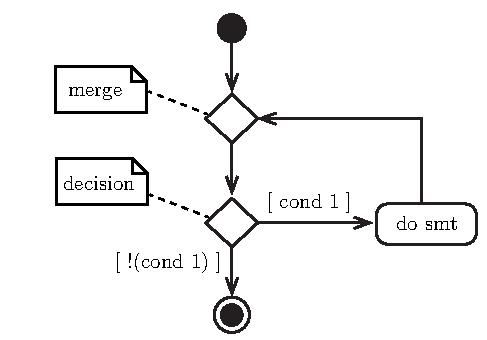
\includegraphics[width=0.50\linewidth]{01_Basics/figures/uml/IterationStatement-00-UML-while.pdf}
% \captionof{figure}{UML \texttt{while} Activity Diagram Representation}
% \label{fig:ch01_Basics_UML_IterationStatement-00-while}
% %~\ref{fig:ch01_Basics_UML_IterationStatement-00-while} 
% %%%%%%%%%%%%%%%%%%%%%%%%%%End figure
% \end{minipage}
% \begin{minipage}{.25\textwidth}
% %%%%%%%%%%%%%%%%%%%%%%%%%%%%%%%%%Begin code
% \begin{lstlisting}[frame=tlrb,numbers=none,mathescape=true,escapechar=\%,columns=flexible]
% some awesome code here
% \end{lstlisting}
% %%%%%%%%%%%%%%%%%%End Code
% \end{minipage}
% \vspace{0.5cm}
% %end minipages


%\begin{enumerate}
%	\item Initialize timer and directions registers
%    \item Specify initial state
%    \item Perform FSM controller
%   \begin{enumerate}
%    	\item Call an output function, which depends on the state
%        \item Delay, which depends on the state
%        \item Call an input function to get the status of the coin sensors
%        \item Change states, which dependes on the state and the input
%    \end{enumerate}
%\end{enumerate}

% \begin{enumerate}
% 	\item Current instruction is finished,
%     \item Eight registers are pushed on the stack,
%     \item LR is set to 0xFFFFFFF9,
%     \item IPSR is set to the interrupt number,
%     \item PC is loaded with the interrupt vector
% \end{enumerate}

% Itemize categoriza poniendo (.) en lugar de números
% \begin{itemize} 
% 	\item I
% 	\item I
% 	\item Y
% 	\item Y
% 	\item Y
% 	\item Y
% 	\item 
% \end{itemize}

% \begin{table}[!h]
% \centering
% \begin{tabular}{|l|l|l|} \hline
% $p$ & bit Field & Interrupt         \\\hline
% $3$ & \bitsRange[31]{29} & Interrupt [$4m+3$]  \\\hline
% $2$ & \bitsRange[23]{21} & Interrupt [$4m+2$]  \\\hline
% $1$ & \bitsRange[15]{13} & Interrupt [$4m+1$]  \\\hline
% $0$ & \bitsRange[7]{5} & Interrupt [$4m$]   \\\hline
% \end{tabular}
% \caption{pasteCaption}
% \label{tab:t_rt_ch04_}
% ~\ref{tab:t_rt_ch04_}
% \end{table}

% Insertar URL
%\url{https://www.osha.gov/Publications/laboratory/OSHAfactsheet-laboratory-safety-noise.pdf}\\

% \newcommand{\bitsRange}[2][50]{\texttt{{#1}-{#2}}}
% \newcommand{\CustomHex}[2][0000]{\texttt{0x{#1}.{#2}}}
% \newcommand{\GPIOPort}[1]{\texttt{GPIO\_PORT{#1}}}
% \newcommand{\GPIOPortR}[2][A]{\texttt{GPIO\_PORT{#1}\_{#2}\_R}}
% \newcommand{\GPIOPortHandler}[1]{\texttt{GPIO\_PORT{#1}\_Handler}}
% \newcommand{\HandlerISR}[1]{\texttt{#1\_Handler}}
% \newcommand{\IRQnr}[1]{\texttt{{#1}}}
% \newcommand{\NVICPRI}[1]{\texttt{NVIC\_PRI{#1}\_R}}
% \newcommand{\NVICEN}[1]{\texttt{NVIC\_EN{#1}\_R}}
% \newcommand{\NVICDIS}[1]{\texttt{NVIC\_DIS{#1}\_R}}
% \newcommand{\Ttimer}[2][A]{\texttt{Timer\_{#2}{#1}}}
% \newcommand{\xNrbit}[1]{$#1$-\texttt{bit}}
% \newcommand{\xNrbits}[1]{$#1$-\texttt{bits}}
% \newcommand{\camouflagegreenCellColor}{\cellcolor[rgb]{0.47, 0.53, 0.42}}
% \newcommand{\lavenderCellColor}{\cellcolor[rgb]{0.9, 0.9, 0.98}}
% \newcommand{\volties}[2][0]{$\si{{#1}\volt}_{#2}$}
% \newcommand{\volti}[1]{$\si{{#1}\volt}$}
% \newcommand{\voltiposi}[1]{$+\si{{#1}\volt}$}
% \newcommand{\voltinega}[1]{$-\si{{#1}\volt}$}